%%%%%%%% ICML 2025 EXAMPLE LATEX SUBMISSION FILE %%%%%%%%%%%%%%%%%

\documentclass{article}

% Recommended, but optional, packages for figures and better typesetting:
\usepackage{microtype}
\usepackage{graphicx}
\usepackage{subfigure}
\usepackage{booktabs} % for professional tables

% hyperref makes hyperlinks in the resulting PDF.
% If your build breaks (sometimes temporarily if a hyperlink spans a page)
% please comment out the following usepackage line and replace
% \usepackage{icml2025} with \usepackage[nohyperref]{icml2025} above.
\usepackage{hyperref}


% Attempt to make hyperref and algorithmic work together better:
\newcommand{\theHalgorithm}{\arabic{algorithm}}

% Use the following line for the initial blind version submitted for review:
% \usepackage{icml2025}

% If accepted, instead use the following line for the camera-ready submission:
\usepackage[accepted]{icml2025}

% For theorems and such
\usepackage{amsmath}
\usepackage{amssymb}
\usepackage{mathtools}
\usepackage{amsthm}

% if you use cleveref..
\usepackage[capitalize,noabbrev]{cleveref}

%%%%%%%%%%%%%%%%%%%%%%%%%%%%%%%%
% THEOREMS
%%%%%%%%%%%%%%%%%%%%%%%%%%%%%%%%
\theoremstyle{plain}
\newtheorem{theorem}{Theorem}[section]
\newtheorem{proposition}[theorem]{Proposition}
\newtheorem{lemma}[theorem]{Lemma}
\newtheorem{corollary}[theorem]{Corollary}
\theoremstyle{definition}
\newtheorem{definition}[theorem]{Definition}
\newtheorem{assumption}[theorem]{Assumption}
\theoremstyle{remark}
\newtheorem{remark}[theorem]{Remark}

% Todonotes is useful during development; simply uncomment the next line
%    and comment out the line below the next line to turn off comments
%\usepackage[disable,textsize=tiny]{todonotes}
\usepackage[textsize=tiny]{todonotes}


% The \icmltitle you define below is probably too long as a header.
% Therefore, a short form for the running title is supplied here:
\icmltitlerunning{Wired Together: Reward-Modulated Hebbian Social Plasticity for Emergent Social Intelligence in Multi-Agent Systems}

\begin{document}

\twocolumn[
\icmltitle{Wired Together: Reward-Modulated Hebbian Social Plasticity \\ for Emergent Social Intelligence in Multi-Agent Systems}

% \icmlsetsymbol{equal}{*}

\begin{icmlauthorlist}
\icmlauthor{Ana Cristiana Marcu}{tu}
\end{icmlauthorlist}

\icmlaffiliation{tu}{Department of Intelligent Systems (INSY) within the Faculty of Electrical Engineering, Mathematics, and Computer Science (EEMCS/EWI), Delft University of Technology}

\icmlcorrespondingauthor{Ana Cristiana Marcu}{acmarcu@tudelft.nl}

\icmlkeywords{Multi-Agent Systems, Multi-Agent Reinforcement Learning, Hebbian Learning, Agent Collaboration}

\vskip 0.3in
]

\printAffiliationsAndNotice{} 
\begin{abstract}
\end{abstract}

\section{Introduction}
\label{intro}

Multi-agent systems (MAS) are increasingly proposed as a substrate for problems that exceed the practical capacity of single-agent learners, such as disaster response, transportation, and large-scale web automation, where parallelism, partial observability, and large scale dynamics are intrinsic to the task \cite{yuan2023survey, wong2023deep}. Multi-Agent Reinforcement Learning (MARL) offers a framework for such systems to learn cooperative joint policies through environmental interaction \cite{yuan2023survey, oroojlooy2023review}, and recent work extends this paradigm to LLM-based agents that integrate planning, memory, and natural-language communication into goal-directed behaviour \cite{xi2025rise, sun2024llm}.

Yet across both lines of work, agents typically treat one another as transient sources of information rather than as enduring partners. Coordination is achieved through learned vector messages \cite{zhu2024survey}, LLM-mediated dialogue \cite{sun2024llm}, or attention over the population \cite{iqbal2019actor}, all recomputed at every step and dissolving when the interaction ends. Self-evolving frameworks soften this by letting agents adapt internal components online \cite{fang2025comprehensive, gao2025survey}, but the population structure itself remains fixed or implicit. The limitation is most consequential in \emph{open environments} where population and tasks shift dynamically \cite{yuan2023survey}, settings that demand persistent social relationships rather than just better per-step coordination \cite{licua2025mindforge}.

Human intelligence offers a model for what is missing. Humans learn not only from direct experience but from one another, and this social learning is what allows knowledge to accumulate across a group rather than being rediscovered by each individual \cite{tomasello1993cultural, hoppitt2013social, boyd2011cultural}. Moreover, social learning is selective: it relies on persistent relationships that determine whom to learn from and what to retain \cite{kendal2018social}. Existing work on social learning between artificial agents \cite{ndousse2021emergent, hillier2024social} captures the act of learning from others but not the persistent bonds that determine whom to learn from over time.

We argue that the missing component in MAS is \emph{structural plasticity at the population level}. Just as the brain's capacity to learn arises not from the intelligence of individual neurons but from the dynamic plasticity of the synapses between them \cite{hebb2005organization, kusmierz2017learning}, a MAS can be viewed as an adaptive network in which inter-agent bonds form the substrate of social intelligence. Under this view, agents play the role of neurons, social bonds play the role of synapses, and reward feedback plays the role of the modulatory signal. We propose that applying a reward-modulated Hebbian rule to inter-agent bonds produces stable social assemblies, meaning pairs and groups of agents that preferentially collaborate, and provides a structural basis for credit propagation, and targeted communication in MAS.

\paragraph{Contributions.} This research makes the following contributions: (i) we formalise a \emph{neuron to agent isomorphism} that maps a MAS to a time-evolving weighted graph governed by a reward-modulated Hebbian rule; (ii) we operationalise the graph through \emph{reward diffusion} across bonded agents and adaptation of partner's beliefs; (iii) we release \emph{Five Chambers}, an open-source Craftium environment with five sequential rooms that require progressively tighter coordination, from solo learning to joint combat; and (iv) we evaluate the framework across a layered comparison of LLM-only agents, LLM agents augmented with a MAPPO RL layer, and the addition of Hebbian Social bonds to the system.
\todo{Here I need to decide what experiments will be added in the end and if I should change this}

\paragraph{Research questions.} We organise our work around four research questions:
\begin{quote}
\textbf{RQ1} Does reward-modulated Hebbian plasticity over inter-agent bonds improve cooperative task performance, compared to LLM-only and RL baselines without a social graph?

\textbf{RQ2} How does the social graph topology evolve over training, and do emergent bond patterns reflect the cooperative structure of the environment?

\textbf{RQ3} Does reward diffusion across the Hebbian graph propagate learning signals across the team, accelerating skill acquisition compared to agents that receive only their own reward?
\end{quote}

\section{Background}
\label{background}

\subsection*{Hebbian learning}
The fundamental capacity of the brain to learn and adapt does not arise from the intelligence of individual neurons, but from the dynamic plasticity of the connections between them. This principle is articulated by Donald Hebb (1949), who proposed that ``cells that fire together, wire together'' \cite{hebb2005organization}. Hebbian theory implies that synaptic strength is increased when the presynaptic cell repeatedly contributes to the firing of the postsynaptic cell, forming the cellular basis of associative learning \cite{brown2020donald, lazari2022hebbian}. The bidirectional refinement of this process is captured by long-term potentiation (LTP), in which co-active synapses are strengthened, and long-term depression (LTD), in which weakly correlated or temporally misaligned activity weakens connections \cite{lazari2022hebbian}.

More recent work extends this to reward-modulated Hebbian plasticity, where synaptic updates also depend on a global modulatory signal (e.g., dopamine) carrying reward or prediction error \cite{kusmierz2017learning}. This three-factor rule allows neural circuits to reinforce only those causal associations that lead to positive outcomes. Through this mechanism, transient neural co-activations stabilise into functional assemblies capable of complex computation.

\subsection*{Social learning}
Human intelligence is fundamentally social: the Social Brain Hypothesis posits that the evolutionary expansion of the primate brain was driven by the computational demands of managing complex, large-scale social relationships \cite{dunbar1998social}. Beyond direct experience, humans rely on social learning to acquire skills and knowledge from one another, allowing groups to outperform any individual member \cite{tomasello1993cultural, boyd2011cultural}. Crucially, social learning is selective rather than indiscriminate: it depends on persistent relationships that determine whom to learn from and what to retain \cite{kendal2018social}.

\subsection*{Dec-POMDPs and cooperative MARL}
Multi-agent environments are formally modelled as Decentralised Partially Observable Markov Decision Processes (Dec-POMDPs) \cite{bernstein2002complexity}. In a Dec-POMDP, $N$ agents act simultaneously in a shared environment under partial observability: each agent $i$ receives a local observation $o_i$, selects an action $a_i$ according to its policy $\pi_{\theta_i}(a_i \mid o_i)$, and receives a reward $r_i$. In the cooperative setting, agents share a common reward signal and the joint objective is to maximise the expected return.

Dec-POMDPs capture the key challenges of real-world multi-agent systems, including partial observability, non-stationarity induced by simultaneous learning, and the need for coordination under limited information \cite{wong2023deep}. Optimal solutions are intractable in general, so most MARL methods approximate Dec-POMDP solutions through centralised training with decentralised execution (CTDE) \cite{amato2015scalable}, in which agents condition value estimates on global information during training while restricting actor inputs to local observations at execution.

\subsection*{Proximal Policy Optimisation (PPO) and MAPPO}
PPO is a policy-gradient method that improves training stability by replacing the standard objective with a clipped surrogate that prevents large parameter updates from destabilising the learned policy \cite{yu2022surprising}. The objective constrains the probability ratio between the new and old policies, ensuring updates remain within a trust region. PPO is augmented with a value-function loss and an entropy bonus that discourages premature convergence to deterministic policies.

Multi-Agent PPO (MAPPO) extends PPO to cooperative MARL under the CTDE paradigm \cite{yu2022surprising}: each agent maintains a local actor that conditions on its observation, while a centralised critic conditions on the joint observation of all agents during training. The critic's advantage estimates account for the team's contribution rather than each agent's individual reward signal.

\subsection*{LLM-based agents}
LLMs have recently been used as the central reasoning core of autonomous agents, mapping structured natural-language observations to discrete actions through prompt-conditioned generation \cite{xi2025rise}. To allow such agents to learn from environmental reward, the LLM is typically frozen and a small set of trainable parameters is added: a classification head that maps a pooled hidden state to a distribution over the action space, and low-rank adapters (LoRA) inserted into the attention layers \cite{hu2022lora}, which constrain the policy update to a low-dimensional subspace and prevent the reward signal from corrupting the LLM's general reasoning capabilities. This paradigm enables policy optimisation against environment reward while preserving the LLM's pre-trained knowledge \cite{qian2025toolrl}.

\section{Related work}
\label{related}

This work draws on three lines of research: prior approaches to coordination in multi-agent learning, the ``neuron as an agent'' paradigm, and Hebbian learning as a mechanism for adaptive behaviour in artificial systems.

\paragraph{Coordination in MARL and LLM-agent systems.} Existing approaches to coordination treat other agents as transient elements of the environment rather than as persistent partners. Three lines of work illustrate this. Model-based auxiliary prediction losses let agents leverage expert behaviour by predicting others' actions \cite{ndousse2021emergent}, but agents minimise the auxiliary objective without forming explicit or lasting relationships, so other agents serve as prediction targets rather than as sources of retained knowledge. Intrinsic motivation methods reward social influence to encourage coordination \cite{jaques2019social}, shaping behaviour without enabling inter-agent skill transfer. Recent Theory of Mind frameworks introduce perspective-taking to improve interpretation of agent intentions \cite{licua2025mindforge}, but enhance reasoning about others rather than learning from them. Across all three, performance gains do not translate into stable social structure \cite{ye2025efficient}.

\paragraph{Neuron as an agent.} A complementary line of research treats individual computational units within a neural network as autonomous, self-interested actors. Early work framed neurons as agents performing Gibbs sampling with synaptic weights modelled as stochastic Gaussian policies \cite{wang2015reinforcement}, and later work used MARL to optimise recurrent networks by viewing neurons as agents that drive the collective system toward rewarded states \cite{chalk2019training}. Other work locate the agent at the synapse rather than the neuron, treating the synapse as the fundamental reinforcement-learning unit responsible for credit assignment \cite{bhargava2022gradient}, or address inter-neuron communication and reward distribution without a trusted third party using auction theory and counterfactual returns \cite{ohsawa2018neuron}. Building on these foundations, \cite{ott2020giving} argues that intelligence emerges bottom-up from the local interactions of self-interested neurons balancing global task rewards against biological incentives. We invert this direction: rather than treating neurons within a network as agents, we treat a population of agents as a network and ask what plasticity rule governs the bonds between them.

\paragraph{Hebbian learning in artificial systems.} Hebbian learning has been used as a local, biologically inspired rule for shaping adaptive behaviour in both neural and multi-agent systems. Prior work leverages Hebbian-style updates to model social factors such as emerging empathy and counter-empathy in agent learning \cite{chen2019reaching}, to perform unsupervised clustering of agents in complex environments such as StarCraft II \cite{kang2023forecasting}, and to build adaptive network models that connect Hebbian plasticity with synchronisation and social bonding dynamics \cite{mukeriia2024multi}. In parallel, Hebbian rules have been explored as a mechanism for robust generalisation, for example by evolving compact shared plasticity rules \cite{pedersen2021evolving} or by meta-learning generalised bidirectional Hebb-style update rules as an alternative to explicit backpropagation \cite{sandler2021meta}. These works apply Hebbian learning either within an agent's internal network or to model behavioural dynamics; we apply it to the inter-agent bond structure itself, treating the population graph as the substrate of plasticity.

\section{Methodology}
\label{methodology}

\subsection*{Environment}
Open environments with shifting populations are the long-term motivation for this framework. Initial pilot experiments using the OpenWorld environment from Craftium \cite{malagoncraftium} confirmed that with a small population and a short horizon, agents rarely encountered one another, so the Hebbian co-activity signal $c_{ij}(t)$ rarely fired and bonds never accumulated. We hypothesise that meaningful Hebbian dynamics in open-world settings require both larger populations and longer horizons. We therefore study the mechanism in a small-population cooperative setting where its effects can be measured in isolation. We introduce \emph{WIRE} (Wired Inter-agent Reasoning Evaluation), a five-stage environment built on Luanti in which agents progress through tasks of increasing coordination demand: solo skill acquisition, joint resource acquisition, a partially observable switch puzzle that can only be solved through targeted communication, and cooperative combat culminating in a boss fight (see \autoref{fig:five_chambers_curriculum}). Each stage builds \emph{mechanism-level interdependence} into the environment itself, so that the value of persistent social bonds can be assessed without needing the population scale that open environments require. WIRE thus serves as a controlled environment for the Hebbian mechanism. A detailed discussion of the environment-selection considerations is provided in \autoref{sec:env_selection}.

\begin{figure*}[t]
    \centering
    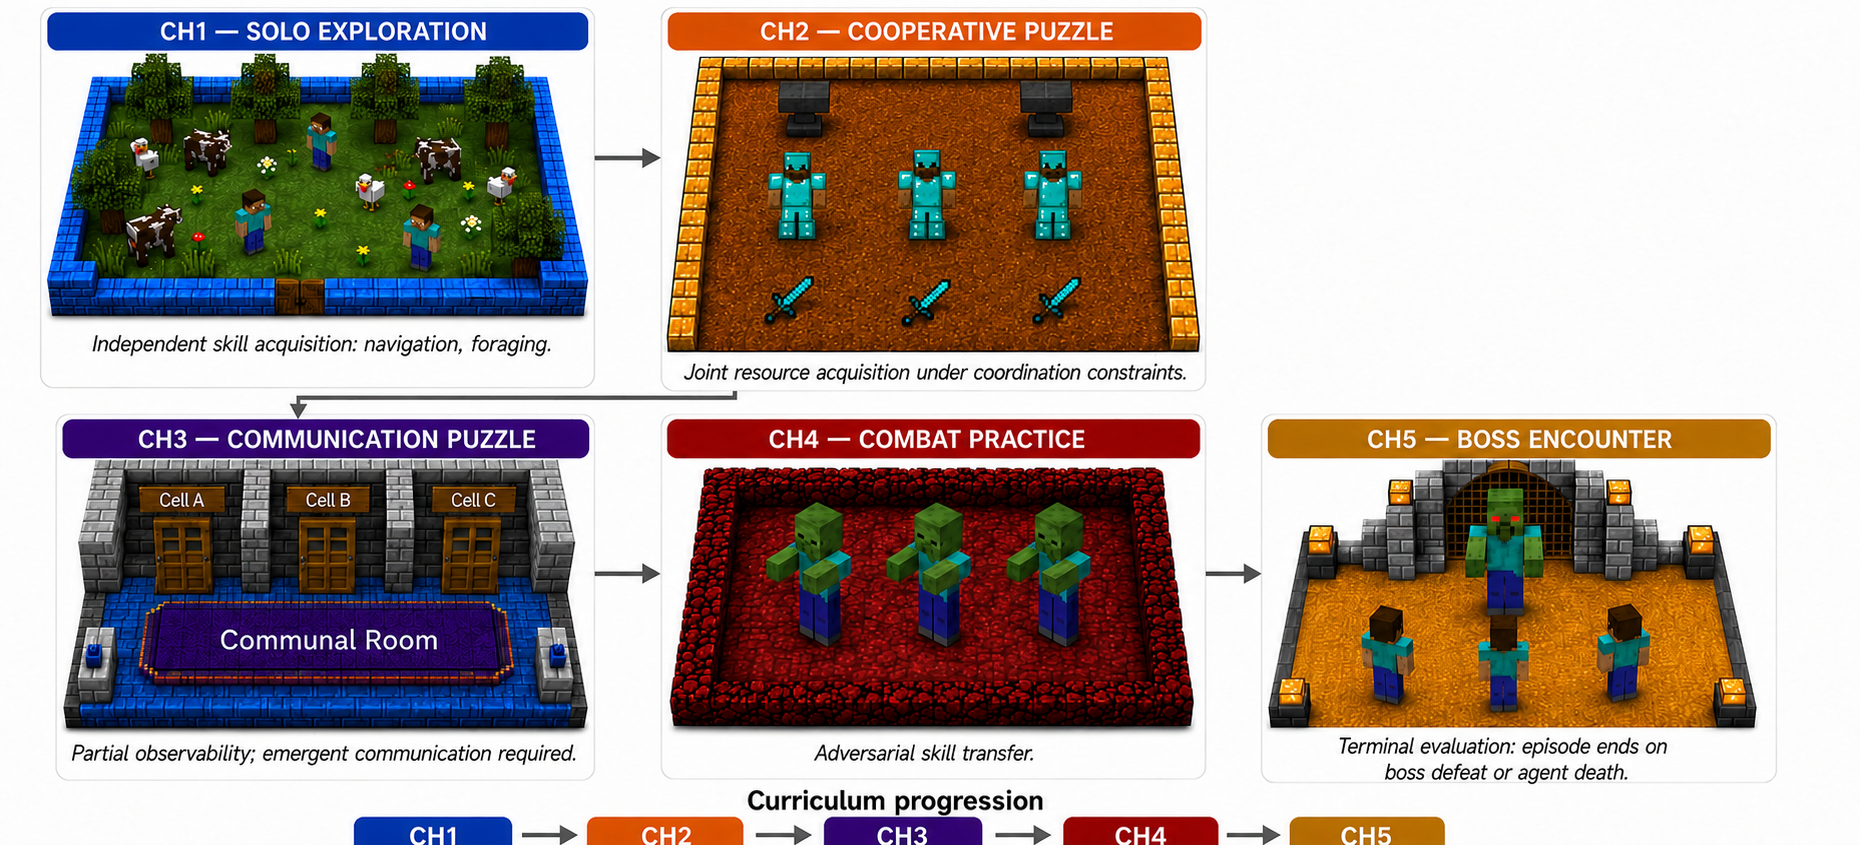
\includegraphics[width=\linewidth]{figures/env_minecraft.png}
    \caption{The WIRE environment (Wired Inter-agent Reasoning Evaluation). Agents progress through five chambers, each targeting a distinct coordination competency: solo skill acquisition (Ch1), cooperative resource acquisition under joint-action requirements (Ch2), targeted communication under partial observability (Ch3), team combat (Ch4), and a cooperative boss fight (Ch5). Episodes terminate on boss defeat or full team death.}
    \label{fig:five_chambers_curriculum}
\end{figure*}

\subsection{Agent architecture}
\label{sec:agent_architecture}

Each agent in WIRE is built on the \emph{MindForge} cognitive stack \cite{licua2025mindforge}: a frozen language model (Qwen3.5-2B throughout) serving as the per-agent reasoning core, augmented with cognitive modules that maintain the agent's situated understanding of the task, its teammates, and its own progress. When the reinforcement-learning layer is enabled, a low-rank adapter (LoRA) \cite{hu2022lora} is inserted into the attention layers and trained against environment reward; the rest of the model remains frozen. At each step, an agent receives a $320 \times 180$ first-person frame, a structured text context, and any messages addressed to it by teammates, and emits one discrete action together with an optional natural-language message addressed to one specific teammate.

\paragraph{Cognitive modules.}
Six modules feed into the action-selection prompt: \emph{perception beliefs} describe what the agent sees in action-relative spatial terms and flag unenacted action--target combinations as intrinsic-motivation targets \cite{georgeon2012interactional}; \emph{partner beliefs} maintain one entry per teammate summarising their chamber, gear, commitments, and reported schemes; \emph{interaction beliefs} extract actionable shared information like role assignments, switch and door status, combat coordination, team-level warnings from recent conversation; \emph{task beliefs} provide a procedural context for the current task, framed as a scheme that pairs an intended action with the observation the agent expects to see; \emph{episodic memory}, a ChromaDB vector store keyed on task embeddings, retrieves past attempts with a 70/30 success-to-failure ratio so the agent sees mostly positive examples without losing failure signal; and \emph{skills} stores successful action-thought pairs in a separate vector store for retrieval on similar tasks.

\paragraph{Auto-curriculum and critic.}
An auto-curriculum module proposes the next concrete task at every step, conditioned on the agent's current chamber, fired milestones, inventory, and a brief question-answer pass. Validity filters reject proposals that reference fixtures outside the agent's current chamber or that contain no actionable keyword, replacing them with a chamber-appropriate fallback. A critic module evaluates task success every twenty steps from the frame, last action, reward, status, inventory, and current task. The verdict drives three downstream effects: successful tasks promote their action into the skill store, repeated failures trigger task reassignment, and every verdict is appended to episodic memory.

\paragraph{Action selection.}
The action-selection prompt is assembled from the frame, current task and context, recent beliefs, retrieved skills and episode summary, live chamber state, inventory, position, status, and a hard-grounded list of chambers the agent has actually visited this episode (the last item rules out a hallucination mode in which the language model claims to be in a chamber it has never entered). The prompt is sent to the base model, which returns a JSON object with action, rationale, message, and target. When the RL policy is active, the LoRA-adapted model produces logits over the discrete action set through a head on the pooled hidden state; an action is sampled and a separate prompt then generates the message conditioned on it. The two-step structure decouples action optimisation (with a clean discrete reward) from message generation (without one).

\paragraph{Action space.}
The action space consists of twenty-two primitives (movement, camera, dig, place, drop, hotbar slot selection) plus four macros: \emph{TurnAround}, \emph{ScanArea}, \emph{ApproachTarget}, and \emph{Escape}. Under reinforcement learning, hotbar-slot actions are masked from the policy because the environment auto-equips the best available tool before each dig; without the mask, slot actions occupied roughly thirty per cent of the action space and the policy collapsed onto slot-selection spam early in training.

\paragraph{Communication.}
All inter-agent communication is targeted: every message specifies a single recipient through a \texttt{communication\_target} field. There is no broadcast channel. The design forces the policy to learn whom to talk to in addition to what to say, the lever the Hebbian social graph is intended to inform. Messages that are too short, identical to the previous message, or sent within two steps of a previous valid message are filtered out and earn no reward. Messages with a malformed target are rerouted to the agent's strongest Hebbian-bonded teammate (or a random teammate when the graph is inactive), but the sender does not earn the per-message reward in this case, so malformed targeting is not positively reinforced.

\subsection{Reinforcement learning formulation}
\label{sec:rl_formulation}

We formulate WIRE as a decentralised partially observable Markov decision process (Dec-POMDP) \cite{bernstein2002complexity} with $N$ homogeneous agents and a shared cooperative reward structure. At each step $t$, agent $i$ observes a tuple $o_i^t$ comprising the visual frame, the structured text context produced by its cognitive modules, and any messages received from teammates; selects a joint output $(a_i^t, m_i^t, \tau_i^t)$ consisting of a discrete action, a natural-language message, and a target teammate for the message; and receives a per-agent reward $r_i^t$. The action $a_i^t$ is drawn from the twenty-six-action space described in the previous subsection.

\paragraph{Policy parameterisation.}
The action policy $\pi_\theta(a \mid o)$ is parameterised by the LoRA-adapted base language model with an action head $\phi$ on the pooled hidden state of the last prompt token. Concretely, the action-selection prompt is tokenised and passed through the model; the final-layer hidden state at the last non-padding position is projected by $\phi$ to logits over the discrete action set, masked to exclude hotbar-slot actions, and normalised by a categorical distribution from which $a_i^t$ is sampled. Only the LoRA parameters and $\phi$ are updated; the base model remains frozen, which constrains the policy update to a low-dimensional subspace and protects the language model's general reasoning capabilities from being corrupted by environment reward \cite{hu2022lora, qian2025toolrl}. Message generation $m_i^t$ uses the same base model in a separate, non-trained call conditioned on the sampled action; the message decision is therefore not part of the policy gradient.

\paragraph{Reward structure.}
The per-agent reward $r_i^t$ is the sum of four streams: (i) a \emph{milestone reward} that fires when a chamber-specific objective is met (M1--M28, ranging from solo skill demonstrations in Chamber 1 to the cooperative boss defeat in Chamber 5; full schedule in \autoref{sec:milestone_table}); (ii) a \emph{communication reward} composed of a base per-message payment for valid messages and a per-chamber communication milestone fired when sustained chat is observed; (iii) a \emph{death penalty} subtracted on termination, so the value baseline learns that dying is worse than running out of steps; and (iv) a small \emph{futile-action penalty} applied when the policy requests a camera tilt past its physical limit, which is the one local validity signal the team-level reward path does not otherwise provide. Communication messages with malformed targets are rerouted but do not earn the base reward, so the gradient does not positively reinforce malformed targeting.

\paragraph{Initial formulation: per-step actor-critic.}
The first experimental track used Multi-Agent PPO (MAPPO) \cite{yu2022surprising} under centralised training with decentralised execution \cite{amato2015scalable}. Each agent runs the policy above with its own LoRA adapter; a single shared critic $V_\psi(s^t)$ conditioned on the joint state baselines the advantage. The joint state is an explicit encoding rather than the raw concatenation of agent observations: per agent, we extract position, current chamber as a one-hot, normalised health, an inventory bag-of-items over the items that drive milestones, a milestone bitmap, and the raw step reward, then concatenate a sentence-transformer embedding of the agent's last action and last message to capture the semantic content the structured features do not. The encoding is fixed-dimensional and shared across agents, so the critic's input layout is stable as agents join or leave (for example through termination).

The policy is updated with the clipped surrogate of PPO \cite{yu2022surprising}; the centralised critic is trained against GAE \cite{} returns on the team-mean reward with the standard PPO value-clipping. Generalised advantage estimation uses the centralised value $V_\psi(s^t)$ as the baseline for each agent's transition; in the IPPO ablation, each agent learns an independent per-agent value head on its own pooled hidden state, with no information sharing across agents at training time.

\paragraph{Pivot to per-trajectory advantage.}
As reported in the experiment log (\autoref{sec:exp_log}), the per-step actor-critic formulation produced reward signals too noisy to push the policy past Chamber 1, with two failure modes traceable to the critic. First, on a sparse-reward five-stage environment the per-step advantage $\delta_t = r_t + \gamma V(s_{t+1}) - V(s_t)$ is dominated by value-function error rather than reward signal whenever $r_t = 0$, which is almost every step. Second, the centralised critic was observed to converge to predicting the team mean, at which point all advantages collapse to noise and the policy gradient is effectively zero. Both modes are inherent to learning a value function in a regime where successful trajectories are rare and the per-step reward variance is small relative to the critic's prediction error.

We therefore replaced the trainer with Group-Relative Policy Optimisation (GRPO). At each update, GRPO samples a group of $G$ joint rollouts of horizon $H$ from the current policy, computes the per-trajectory return $R_g = \sum_{t=0}^{H-1} \gamma^t r_t^{(g)}$ for each rollout $g$, and assigns the group-relative advantage
\[
A_g \;=\; R_g - \frac{1}{G}\sum_{g'=1}^{G} R_{g'}
\]
to every transition within rollout $g$. The clipped surrogate is then applied to update the LoRA adapter, with KL regularisation against a frozen reference adapter to keep the policy near its initialisation. Two properties of this scheme matter for our setting. The advantage is per-trajectory rather than per-step, which is the natural granularity for an environment where reward is sparse and milestone-driven; whether a rollout fired a milestone or not is information the gradient sees directly, without having to be reconstructed from a learned value function. And the group baseline removes the need for a learned critic entirely, which eliminates both failure modes of the per-step formulation at once.

\paragraph{Coupling to the Hebbian graph.}
GRPO admits two natural insertion points for the Hebbian module, described in detail in the following subsection. \emph{Reward diffusion} redistributes per-step rewards along the current bond matrix before the trajectory return $R_g$ is computed, so a strongly bonded teammate's success enters the agent's gradient as its own. \emph{Group composition} replaces some of the $G$ trajectories that the relative baseline averages over with trajectories borrowed from co-bonded peers, treating the policy update as if the group included imagined samples from the agent's social neighbourhood. The two mechanisms operate on different parts of the GRPO loss, diffusion changes the return, composition changes the sample distribution, and are evaluated in isolation as well as in combination so that any gain can be attributed to the correct axis.


\subsection{Hebbian social plasticity}
\label{sec:hebbian_method}

The core mechanism is a learned weighted graph over agents whose edges are updated by a reward-modulated Hebbian rule. The graph is parameter-free in the conventional sense: nothing about it is back-propagated, and its updates come from a fixed local rule with hyperparameters fixed at the start of training.

\paragraph{The social graph.}
Let $\mathbf{W}(t) \in [0, 1]^{N \times N}$ be the directed social graph at step $t$, with $W_{ij}(t)$ representing agent $i$'s learned trust or attention toward agent $j$. The diagonal is held at zero and the graph is initialised at $W_{ij}(0) = w_0$ for all $i \neq j$, a small positive warm-start value so that reward-diffusion and weighted-sharing mechanisms have something to operate on from the first step. The graph is directed: $W_{ij}$ and $W_{ji}$ evolve independently, which lets the model express asymmetric social relations.

\paragraph{Co-activity signal.}
The Hebbian rule fires when two agents are jointly active at the same step. We define the co-activity signal $c_{ij}(t) \in [0, 1]$ as the product of a spatial gate and an engagement score, augmented by a communication bonus that allows agents to be co-active across distance when they exchange messages:
\[
g_i(t) \;=\; \mathrm{clip}\!\Big(\alpha \, \frac{|r_i(t)|}{r_{\max}} \,+\, (1 - \alpha) \, \mathds{1}[i \text{ communicates}],\; 0,\; 1\Big),
\]
\[
c^{\text{spat}}_{ij}(t) \;=\; \mathds{1}\!\big[\|\mathbf{p}_i(t) - \mathbf{p}_j(t)\| \le d\big] \cdot g_i(t) \, g_j(t),
\]
\[
c^{\text{comm}}_{ij}(t) \;=\; \delta_{\text{comm}} \cdot \mathds{1}[i \leftrightarrow j] \cdot \big(1 - \mathds{1}[\|\mathbf{p}_i - \mathbf{p}_j\| \le d]\big),
\]
\[
c_{ij}(t) \;=\; \mathrm{clip}\!\big(c^{\text{spat}}_{ij}(t) + c^{\text{comm}}_{ij}(t),\; 0,\; 1\big).
\]
The engagement score $g_i(t)$ is high when agent $i$ is either receiving non-trivial reward or actively communicating; $r_{\max}$ is a running maximum of observed absolute rewards used to keep the score scale-invariant. The spatial term $c^{\text{spat}}_{ij}$ fires only for pairs that are within interaction radius $d$ and both engaged. The communication term $c^{\text{comm}}_{ij}$ captures the case where two agents communicate but are not co-located, preventing double-counting when they are.

\paragraph{Modulatory signal.}
Each agent computes a scalar modulator $m_i(t)$ that captures whether it
did well or badly on this step. Where available, $m_i$ is derived from the
per-step advantage $A_i(t) = r_i(t) - V(s_i(t))$; otherwise it falls back
to the normalised step reward. The modulator decomposes into long-term
potentiation (LTP, bond growth) and long-term depression (LTD, bond decay)
terms with separate learning rates, reflecting the biological observation
that strengthening and weakening synapses are governed by different
processes \cite{lazari2022hebbian}:
\[
m^{\text{LTP}}_i(t) \;=\; \eta_+ \tanh\!\big(\beta \max(A_i(t), 0)\big),
\]
\[
m^{\text{LTD}}_i(t) \;=\; \eta_- \tanh\!\big(\beta \max(-A_i(t) - \theta_{\text{LTD}}, 0)\big),
\]
\[
m_i(t) \;=\; m^{\text{LTP}}_i(t) - m^{\text{LTD}}_i(t).
\]
The threshold $\theta_{\text{LTD}}$ is the methodological consequence of asymmetry: small-negative advantages produced by exploration noise on zero-reward steps would, without the threshold, slowly depress every bond regardless of whether the team is genuinely failing. With the threshold, LTD fires only when the agent's signal is clearly negative. The egocentric form ($m_i$ depends only on agent $i$'s own signal) means that when agent $i$ succeeds, all of its outgoing bonds toward currently co-active partners strengthen. Differentiation across partners comes from the co-activity gate $c_{ij}$, not from the modulator.

\paragraph{Sustained co-failure.}
A rolling window of length $T_F$ tracks which pairs have been co-active during team-level failure steps, defined as steps where the team-mean advantage $\bar{A}(t)$ falls below $-\theta_{\text{LTD}}$. Letting $F_{ij}(t) \in [0, 1]$ be the fraction of recent failure steps the pair $(i, j)$ shared, the sustained LTD term is
\[
\Delta W^{\text{LTD,sus}}_{ij}(t) \;=\; -\lambda_F \cdot F_{ij}(t) \cdot W_{ij}(t),
\]
which depresses a bond proportionally to how often the pair has recently been jointly active during failure. The team-mean threshold is intentional: sustained LTD tracks situations where the whole team is repeatedly co-failing, which is a team-level signal rather than a per-pair one.

\paragraph{Failure-tolerant LTP.}
Sustained LTD captures the desired long-run dynamic but produces an early-training pathology: the first few attempts at any cooperative task have a high probability to fail, and the sustained-LTD term collapses
early bonds before they have a chance to consolidate. We introduce a
failure-tolerant LTP term that counteracts this in the early phase. When
the team is failing but the pair's failure co-activation $F_{ij}$ is still
below a tolerance threshold $F_{\text{tol}}$, an additive LTP bonus is
applied that fades linearly to zero as $F_{ij}$ approaches the threshold:
\[
\rho_{ij}(t) \;=\; \mathrm{clip}\!\Big(1 - \frac{F_{ij}(t)}{F_{\text{tol}}},\; 0,\; 1\Big),
\]
\begin{align*}
\Delta W^{\text{tol}}_{ij}(t) \;=\;\; & \eta_F \cdot \rho_{ij}(t) \cdot c_{ij}(t) \cdot \big(1 - W_{ij}(t)\big), \\
                                       & \text{when } \bar{A}(t) < -\theta_{\text{LTD}}.
\end{align*}
The semantic content of the term is: \emph{we tried something together and
it did not work, so the partnership is reinforced for trying; if we keep
failing together, the bonus fades and sustained LTD takes over}. The
failure-tolerant term and the sustained-LTD term operate on the same
statistic $F_{ij}$ but in opposite directions, sustained LTD subtracts
in proportion to $F_{ij}$, while the tolerant term adds in proportion to
$\rho_{ij} = 1 - F_{ij}/F_{\text{tol}}$, together implementing a
per-pair window that rewards co-activity during early shared failure and
prunes it during sustained shared failure. Without this counter-measure,
we observed the bond matrix collapsing to near-zero across the early
phase of training before any cooperative milestone could fire.


\paragraph{The full update.}
Combining the four components above with a passive decay term gives the
full update rule shown in Eq.~\eqref{eq:hebbian_full_update}, followed by
a clip that keeps each bond in $[0, 1]$.

\begin{figure*}[t]
\begin{equation}
\label{eq:hebbian_full_update}
\Delta W_{ij}(t) \;=\;
\underbrace{m_i(t) \cdot c_{ij}(t) \cdot \big(1 - W_{ij}(t)\big)}_{\text{advantage-gated LTP/LTD}}
\,+\, \underbrace{\eta_0 \cdot c_{ij}(t) \cdot \big(1 - W_{ij}(t)\big)}_{\text{base co-activity LTP}}
\,-\, \underbrace{\lambda \cdot W_{ij}(t)}_{\text{passive decay}}
\,+\, \underbrace{\Delta W^{\text{LTD,sus}}_{ij}(t)}_{\text{sustained LTD}}
\,+\, \underbrace{\Delta W^{\text{tol}}_{ij}(t)}_{\text{failure-tolerant LTP}}
\end{equation}
\end{figure*}

\noindent
\[
W_{ij}(t+1) \;=\; \mathrm{clip}\!\big(W_{ij}(t) + \Delta W_{ij}(t),\; 0,\; 1\big).
\]
The five terms in Eq.~\eqref{eq:hebbian_full_update} operate at different
time-scales and respond to different signals. The advantage-gated term is
the primary reward-driven signal: it grows or shrinks the bond in
proportion to agent $i$'s own success, gated by current co-activity. The
base co-activity LTP, with $\eta_0 \ll \eta_+$, is a small unconditional
growth term that fires whenever a pair is co-active regardless of reward
sign. It provides a floor against pure decay so that co-presence alone
slowly builds bonds in the absence of clear reward signal. Passive decay
applies a uniform pull toward zero on every step, so bonds that are not
actively reinforced fade. Sustained LTD and the failure-tolerant LTP form the matched
pair described earlier, operating on the same statistic $F_{ij}$ but with
opposite polarity to implement a per-pair tolerance window. The
$(1 - W_{ij})$ factor on all three LTP terms is a saturation gate that
diminishes growth as bonds approach unity, bounding the matrix from above
without relying on the final clip; the clip itself serves only as a safety
rail against the LTD terms pushing bonds below zero.

\paragraph{Couplings to the RL loop.}
The graph influences the policy update through two mechanisms. Both operate downstream of the update rule above and neither modifies how the graph itself evolves.

\emph{Reward diffusion.} Before the trajectory return is computed, the per-agent reward $r_i(t)$ is replaced by a Hebbian-blended version that incorporates a $\overline{W}$-weighted average of teammate rewards:
\[
r'_i(t) \;=\; (1 - \gamma) \, r_i(t) \,+\, \gamma \sum_{j \neq i} \overline{W}_{ij}(t) \, c_{ij}(t) \, r_j(t),
\]
where $\overline{W}_{ij}(t) = W_{ij}(t) / \sum_{k \neq i} W_{ik}(t)$ is the row-normalised graph and $\gamma$ is the diffusion strength. The co-activity gate $c_{ij}$ inside the sum ensures that reward only flows along bonds that are currently active. The trajectory return that the policy gradient sees is computed from the diffused rewards, so a teammate's success enters the agent's gradient as its own, weighted by how strongly the agent attends to that teammate.

% \emph{Group composition.} For GRPO updates, the group of trajectories $\{\tau_1, \ldots, \tau_G\}$ over which the relative baseline $\bar{R} = \tfrac{1}{G} \sum_g R(\tau_g)$ is computed is augmented with trajectories \emph{borrowed} from co-bonded teammates. A fraction $\kappa$ of the group is replaced by samples drawn from teammate $j$'s rollout buffer with probability proportional to $\overline{W}_{ij}$. The clipped surrogate of GRPO provides the off-policy correction for the borrowed samples without an explicit importance-sampling factor. Where reward diffusion changes the \emph{value} of each trajectory in the group, group composition changes the \emph{identity} of the trajectories the group contains. The two mechanisms therefore enter the GRPO loss at different points and admit clean isolation in the experimental design.

% \paragraph{Properties of the rule.}
% The combined update has three properties worth flagging for the analysis that follows. \emph{Boundedness} is guaranteed by the saturation gates on the LTP terms and the clip on the final weight, so $W$ stays in $[0, 1]^{N \times N}$ without any explicit normalisation step. \emph{Asymmetry} is preserved because the modulator is egocentric and the failure-window snapshot is symmetric only in the sense that it tracks pairs, not in the sense that it equates $W_{ij}$ with $W_{ji}$; either bond can grow or collapse independently. \emph{Locality} is preserved in the sense that each $W_{ij}$ update depends only on the per-agent signals of $i$ and $j$, their pairwise co-activity, and the team-mean advantage, there is no global parameter optimisation step.

\subsection*{Communication protocol}
\subsection*{Metric}

\subsection*{Experimental conditions}


\section{Results}
\label{results}

\section{Discussion }
\label{disc}
\subsection{Limitations}
\subsection{Future Work}
\subsection{Societal Implications}

\section{Conclusion}
\label{concl}


\bibliography{example_paper}
\bibliographystyle{icml2025}


%%%%%%%%%%%%%%%%%%%%%%%%%%%%%%%%%%%%%%%%%%%%%%%%%%%%%%%%%%%%%%%%%%%%%%%%%%%%%%%
%%%%%%%%%%%%%%%%%%%%%%%%%%%%%%%%%%%%%%%%%%%%%%%%%%%%%%%%%%%%%%%%%%%%%%%%%%%%%%%
% APPENDIX
%%%%%%%%%%%%%%%%%%%%%%%%%%%%%%%%%%%%%%%%%%%%%%%%%%%%%%%%%%%%%%%%%%%%%%%%%%%%%%%
%%%%%%%%%%%%%%%%%%%%%%%%%%%%%%%%%%%%%%%%%%%%%%%%%%%%%%%%%%%%%%%%%%%%%%%%%%%%%%%
\newpage
\appendix
\onecolumn
\section{Environmment selection}
\label{sec:env_selection}

\section{Environment selection}
\label{sec:env_selection}

The choice of environment is consequential because progress in RLlearning is closely coupled to the affordances and limitations of the simulator used. Classic platforms such as the Arcade Learning Environment enabled breakthroughs like DQN on Atari games, while more recent work on embodied and open-ended agents relies on visually rich 3D worlds such as Minecraft-based MineDojo. These environments expose a fundamental trade-off: researchers must often choose between computationally efficient but overly simplistic settings (e.g.\ small 2D gridworlds) and substantially slower but richer 3D simulators. Many of the richest environments are also built on closed-source commercial games such as Minecraft, which limits how much their mechanics can be modified or extended.

A second limitation is the lack of flexibility. Commonly used benchmarks either restrict customisation or require specifying environments in complex domain-specific languages, and many only support 2D worlds. This makes it difficult to design targeted scenarios for analysing specific behaviours such as long-horizon cooperation, coalition formation, or persistent social structure.

\paragraph{Why Craftium.} Craftium \cite{malagoncraftium} is a fully open-source 3D voxel world built on the Minetest game engine, supporting both single- and multi-agent scenarios through standard Gymnasium and PettingZoo interfaces. It is explicitly designed for rich 3D navigation, building, and resource-collection tasks, remains computationally efficient compared to Minecraft-based frameworks, and is highly customisable via a Lua API.\footnote{See \cite{malagoncraftium} for benchmarks and examples of single- and multi-agent tasks, open-world survival scenarios, and procedurally generated continual-learning curricula.} Its main drawback is that it is a framework rather than a fixed benchmark: additional engineering effort is required to design, implement, and validate specific social scenarios.

\paragraph{From OpenWorld to Five Chambers.} Our initial design used Craftium's OpenWorld environment with three heterogeneous roles (Engineer, Hunter, Guardian) corresponding to the three skill tracks (tools, hunt, defend). Pilot runs revealed that at small population sizes and short horizons, agents rarely co-located in shared regions, so co-activity signals required by the Hebbian update rule did not fire often enough for bonds to form. We considered scaling up the population and episode length to address this, but the compute requirements quickly exceeded the computation available for this research. We therefore designed \emph{Five Chambers}: a curriculum that retains Craftium's voxel-world affordances (3D navigation, resource collection, combat) but enforces co-location and shared task progression at every stage, so that the Hebbian mechanism can be evaluated under conditions where co-activity is reliably present. This environment structure now introduces more opportunities for collaboration, reducing the need for a longer horizon. Studying the mechanism at scale in genuinely open environments remains an open direction.

% \section{Experiment log}
% \label{sec:exp_log}

% The experimental track for this thesis evolved substantially as evidence accumulated about what the Five Chambers environment, the Hebbian hypothesis, and the available compute could jointly support. This section records the methodological choices and the rationale behind each pivot, so that the contribution of the final experimental design can be read against the alternatives considered.

% \paragraph{Initial experiment.}
% The first experimental track combined three parts: a MindForge-style LLM agent as the per-agent reasoning core, a multi-agent actor-critic learner (MAPPO with a shared centralised critic, with IPPO as an ablation) that fine-tuned a LoRA adapter on top of the frozen base, and the Hebbian social-plasticity graph. The choice reflected the thesis's position relative to prior work: the Hebbian graph is proposed as an augmentation of existing cooperative MARL methods, not a replacement for them. The experimental grid was sized accordingly: model-axis baselines, communication on/off, Hebbian on/off, and a population-scaling sweep at three, six, and nine agents.


% \paragraph{What the initial experiment revealed.}
% Runs through this stack converged on the same ceiling. Agents plateaued at Chamber 1 across every condition, regardless of whether the reinforcement learner or the Hebbian module was active; the furthest skill-driven milestone was a Chamber 1 pickup task. Subsequent chambers were entered only through a timeout teleport added to prevent indefinite stalls in solo learning. In the runs that combined reinforcement learning with Hebbian shaping, per-agent returns were unequal: a single agent dominated task reward while its teammates trended net-negative. The bond matrix that the Hebbian module was meant to grow instead collapsed, with mean bond strength falling from its warm-start value to near zero. The reason was structural rather than algorithmic: the rule's co-activity input was empty for agents that never co-engaged.

% This made the core hypothesis untestable in this stack. The thesis claim is that reward-modulated Hebbian plasticity over inter-agent bonds builds useful social structure; verifying or refuting that requires agents to co-engage often enough for the rule to fire. With agents stuck in solo skills in Chamber 1, there was no co-activity to reinforce. The aggregated cooperation score, intended as a summary statistic, was correspondingly uninformative, it sat near its noise floor regardless of behaviour and could only meaningfully report deltas, not absolute levels.

% \paragraph{Isolating the Hebbian representation from the gradient.}
% Before moving on, we ran two inference-time-only studies that address a different and methodologically cleaner question: when the language model is not trained at all, does the Hebbian representation alone improve coordination? The first variant surfaces the current bond matrix as a social-context block in the system prompt; the second additionally surfaces the rewards a teammate's actions have just propagated to the agent. Both variants disable the reinforcement-learning gradient entirely. If either condition outperforms the plain language-model baseline, the Hebbian representation has signal that does not depend on a successful gradient path; if both match the baseline, the contribution must flow through the optimiser instead. These runs are inexpensive, isolate a question the gradient-driven experiments cannot, and remain part of the final experimental matrix regardless of how the policy-optimisation track resolves.

% \paragraph{Pivoting to group-relative policy optimisation.}
% From the first experiments we learnt that the per-step actor-critic learning was producing too noisy a gradient signal on a sparse-reward, five-stage environment to push the policy past Chamber 1. Second, the centralised critic itself was a plausible cause of the agent-domination pattern, since one over-represented learner can pull the shared value baseline toward its own returns and starve teammates of advantage signal. We therefore replaced the trainer with Group-Relative Policy Optimisation (GRPO). The relevant property for our purposes is not that GRPO is newer, but that it removes both failure modes at once: each update is scored against a baseline computed from a group of trajectories sampled from the same policy, so no learned critic is needed; and the advantage is per-trajectory rather than per-step, which is the natural granularity for an environment where reward is sparse and milestone-driven. A practical side benefit is that the Hebbian augmentation has a clean place to attach inside the GRPO loop, which the next paragraph develops.

% \paragraph{Decomposing the Hebbian contribution into two mechanisms.}
% Once a working trainer was in place, the temptation was to combine all Hebbian machinery into a single condition and compare it against the unaugmented baseline. We chose not to. The Hebbian module enters the GRPO loop through two orthogonal mechanisms that operate on different parts of the loss. \emph{Reward diffusion} redistributes per-step rewards along the current bond matrix before the trajectory return is computed, so a strongly bonded teammate's success enters the gradient as the agent's own. \emph{Group composition} replaces some of the trajectories that the group-relative baseline averages over with trajectories borrowed from co-bonded peers, treating the policy update as if the comparison group included imagined samples drawn from the agent's social neighbourhood. A combined condition that turned both mechanisms on at once would conflate them: if the combination outperformed the baseline, we could not say which mechanism carried the gain, nor rule out that one helped while the other cancelled. We therefore evaluate each axis in isolation, then together, with the explicit position that a negative result on either axis is as informative for the methodological contribution as a positive one.

\section{Milestone reward schedule}
\label{sec:milestone_table}

The per-agent reward stream $r_i^t$ described in Section~\ref{sec:rl_formulation} is driven primarily by a milestone ladder embedded in the WIRE environment. Milestones are fired by a Lua-side event system in the Luanti server, which writes to an event log polled by the Python training loop each step. When a milestone fires, its reward is credited to one or more \emph{contributors} --- the agents whose action triggered the event, and propagated through the Hebbian reward-diffusion mechanism before being passed to the policy update.

\paragraph{Track structure.}
Milestones are organised into six tracks. The first five correspond to the five chambers and scale in reward with the coordination demand of the chamber: Chamber 1 milestones reward solo skill demonstrations and pay between 10 and 80 points each; Chamber 2 milestones reward cooperative resource acquisition at the anvils and pay 30--50 points; Chamber 3 milestones reward the switch puzzle resolution and team regrouping (20--100 points); Chamber 4 milestones reward team combat (30--150 points); and Chamber 5 milestones reward the boss fight, with the largest single payouts in the schedule (50--300 points) reflecting both the difficulty of the encounter and the fact that it is the terminal objective. The sixth track is the \emph{communication track}, which provides a per-chamber reward when an agent sustains valid targeted communication in that chamber; it is structurally separate from the chamber-progress tracks so that the contribution of communication to the policy gradient can be ablated cleanly.

\paragraph{Co-completion and contributor credit.}
Several milestones (M19, M22, M23, M27, M28) are inherently team-level events: they fire once when a global condition is met (all agents in the communal room, all mobs killed, boss defeated, etc.) rather than per-agent. For these, the event log records all agents currently contributing to the condition as contributors, and the per-milestone reward is split equally across them at the metric layer; for the post-hoc cooperation analysis, damage-share credit rules are applied to combat milestones so that contribution shares track actual damage dealt rather than just presence. The per-agent reward delivered to the policy gradient at runtime, however, is the full milestone value, not the split share, the split is a post-hoc analytical construct.

\paragraph{Communication reward.}
The communication track is delivered through a separate mechanism. Each valid message earns a small base payment, capped at a per-agent per-episode total to prevent reward farming through chat spam; in addition, when an agent emits more than a threshold number of valid messages in a single chamber, that chamber's communication milestone fires once. Validity rules (minimum length, no duplicates, rate-limited) and target-validity rules (no self-targeting, no broadcast, no missing target) gate both rewards: messages that fail validity earn nothing, and messages with malformed targets are rerouted but their sender does not receive the base reward.

\paragraph{Auxiliary penalties.}
Two negative reward components are applied outside the milestone schedule. A death penalty (--50 points) is subtracted when an agent terminates, so the value baseline learns that dying mid-episode is worse than running out of steps with the team intact. 

\paragraph{Full schedule.}
Table~\ref{tab:milestone_schedule} lists every milestone, its firing condition, and its reward value. Reward magnitudes were chosen iteratively during environment development with the design constraint that (i) the cumulative reward attainable from a chamber should grow as the cooperation demand of that chamber grows, so a team that successfully completes Chamber 5 receives substantially more reward than one that only completes Chamber 1; (ii) within a chamber, milestones should be ordered such that early milestones serve as stepping stones for later ones, with reward magnitudes signalling the relative progress they represent; and (iii) the communication track should be large enough to be a non-trivial part of the policy gradient but small enough not to dominate it.

\begin{table*}[t]
\centering
\caption{Full milestone reward schedule for the WIRE environment. \emph{Type} denotes whether the milestone fires per-agent (P) or as a team-level event (T). \emph{Trigger} summarises the firing condition; full conditions are encoded in the Lua-side event system.}
\label{tab:milestone_schedule}
\small
\begin{tabular}{lllrl}
\toprule
ID & Track & Trigger & Reward & Type \\
\midrule
\multicolumn{5}{l}{\emph{Chamber 1 --- solo skill acquisition}} \\
M1  & ch1\_solo     & Move more than 5 blocks from spawn      & 10   & P \\
M2  & ch1\_solo     & Dig any 3 blocks                        & 30   & P \\
M3  & ch1\_solo     & Pick up 3 dropped items                 & 30   & P \\
M4  & ch1\_solo     & Dig 5 wood blocks                       & 50   & P \\
M5  & ch1\_solo     & Kill 1 animal                           & 50   & P \\
M6  & ch1\_solo     & Kill 2 animals                          & 80   & P \\
M7  & ch1\_solo     & Dig 3 stone blocks                      & 60   & P \\
\midrule
\multicolumn{5}{l}{\emph{Chamber 2 --- cooperative resource acquisition}} \\
M8  & ch2\_anvils   & Break anvil A1 (Row A, position 1)       & 40   & T \\
M9  & ch2\_anvils   & Break anvil A2 (Row A, position 2)       & 40   & T \\
M10 & ch2\_anvils   & Break anvil A3 (Row A, position 3)       & 40   & T \\
M11 & ch2\_anvils   & Break anvil B1 (Row B, position 1)       & 40   & T \\
M12 & ch2\_anvils   & Break anvil B2 (Row B, position 2)       & 40   & T \\
M13 & ch2\_anvils   & Break anvil B3 (Row B, position 3)       & 40   & T \\
M14 & ch2\_anvils   & Diamond sword auto-equipped              & 50   & P \\
M15 & ch2\_anvils   & Diamond chestplate auto-equipped         & 30   & P \\
\midrule
\multicolumn{5}{l}{\emph{Chamber 3 --- communication under partial observability}} \\
M16 & ch3\_switches & Enter isolation cell                     & 20   & P \\
M17 & ch3\_switches & Press cell switch                        & 40   & P \\
M18 & ch3\_switches & Cell door opened by teammate's switch    & 60   & P \\
M19 & ch3\_switches & All agents in communal room              & 100  & T \\
\midrule
\multicolumn{5}{l}{\emph{Chamber 4 --- team combat}} \\
M20 & ch4\_combat   & Enter Chamber 4                          & 30   & P \\
M21 & ch4\_combat   & First mob kill                           & 60   & P \\
M22 & ch4\_combat   & All mobs killed                          & 150  & T \\
M23 & ch4\_combat   & All agents alive after Ch4 cleared       & 100  & T \\
\midrule
\multicolumn{5}{l}{\emph{Chamber 5 --- cooperative boss fight}} \\
M24 & ch5\_boss     & Enter Chamber 5                          & 50   & P \\
M25 & ch5\_boss     & First damage dealt to boss               & 80   & P \\
M26 & ch5\_boss     & Boss at 50\% health                      & 120  & T \\
M27 & ch5\_boss     & Boss defeated                            & 300  & T \\
M28 & ch5\_boss     & All agents alive at boss defeat          & 250  & T \\
\midrule
\multicolumn{5}{l}{\emph{Communication track}} \\
M\_comm\_ch1 & comm  & Sustained valid messaging in Chamber 1   & 40   & P \\
M\_comm\_ch2 & comm  & Sustained valid messaging in Chamber 2   & 20   & P \\
M\_comm\_ch3 & comm  & Sustained valid messaging in Chamber 3   & 30   & P \\
M\_comm\_ch4 & comm  & Sustained valid messaging in Chamber 4   & 15   & P \\
M\_comm\_ch5 & comm  & Sustained valid messaging in Chamber 5   & 20   & P \\
\bottomrule
\end{tabular}
\end{table*}


\section{Use of AI}
%%%%%%%%%%%%%%%%%%%%%%%%%%%%%%%%%%%%%%%%%%%%%%%%%%%%%%%%%%%%%%%%%%%%%%%%%%%%%%%
%%%%%%%%%%%%%%%%%%%%%%%%%%%%%%%%%%%%%%%%%%%%%%%%%%%%%%%%%%%%%%%%%%%%%%%%%%%%%%%


\end{document}
